\section{Resultados}

\subsection{Módulos implementados}
Los resultados muestran la implementación exitosa de todos los módulos planificados:

\begin{enumerate}
    \item \textbf{Autenticación y perfiles}: Sistema de login con JWT; renovaciones de token; recuperación de contraseña; perfil del empleado con datos personales, área/cargo/ubicación y contrato activo \cite{estudio_aplicaciones_java}\cite{analisis_google_charts}\cite{gestion_talento_digital}.
    \item \textbf{Asistencia}: Registro de entrada/salida, cálculo de horas trabajadas, gestión de turnos \cite{estudio_aplicaciones_java}\cite{analisis_google_charts}\cite{gestion_talento_digital}.
    \item \textbf{Permisos e incapacidades}: Solicitud con tipo, fechas, motivo y adjuntos; flujo de estados; observaciones \cite{estudio_aplicaciones_java}\cite{analisis_google_charts}\cite{gestion_talento_digital}.
    \item \textbf{Capacitaciones/inducción}: Asignación de contenidos, evaluaciones, seguimiento de avances y registro de participación \cite{estudio_aplicaciones_java}\cite{analisis_google_charts}\cite{gestion_talento_digital}.
    \item \textbf{Contratos}: Catálogo de tipos, fechas de inicio/fin, renovaciones y alertas por proximidad a vencimiento \cite{estudio_aplicaciones_java}\cite{analisis_google_charts}\cite{gestion_talento_digital}.
    \item \textbf{Certificados}: Generación de certificados laborales con datos parametrizables \cite{estudio_aplicaciones_java}\cite{analisis_google_charts}\cite{gestion_talento_digital}.
    \item \textbf{Reportes y visualizaciones}: Indicadores operativos y tendencias de asistencia/permisos \cite{estudio_aplicaciones_java}\cite{analisis_google_charts}\cite{gestion_talento_digital}.
    \item \textbf{Auditoría y seguridad}: Registro de acciones (crear/actualizar/eliminar), control de roles y verificación de integridad \cite{estudio_aplicaciones_java}\cite{analisis_google_charts}\cite{gestion_talento_digital}.
\end{enumerate}

La \cref{fig:metricas_dora} presenta las estadísticas de permisos registrados por tipo.

\begin{figure}[htbp]
    \centering
    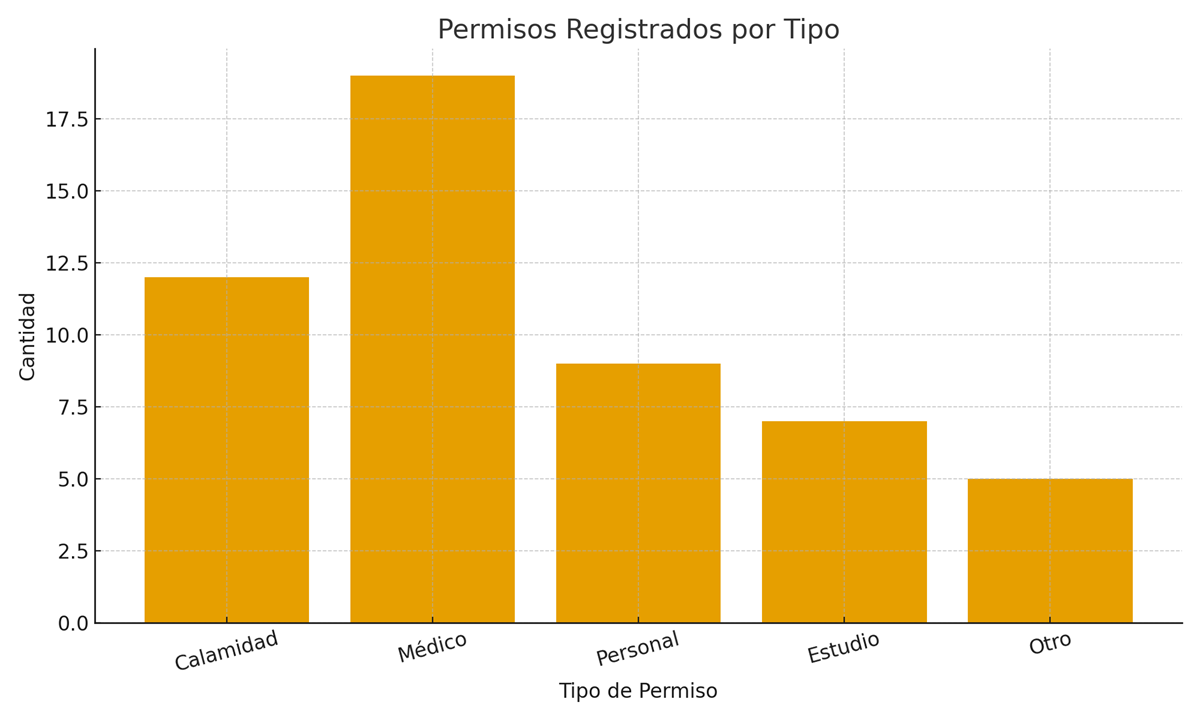
\includegraphics[width=0.48\textwidth]{graphics/permisosregistrados.png}
    \caption{Permisos registrados por tipo}
    \label{fig:metricas_dora}
\end{figure}

\subsection{Evolución temporal de métricas}
Observamos una mejora en la eficiencia de procesos de RRHH. La \cref{fig:evolucion_metricas} muestra las estadísticas de emisión de certificados por mes.

\begin{figure}[htbp]
    \centering
    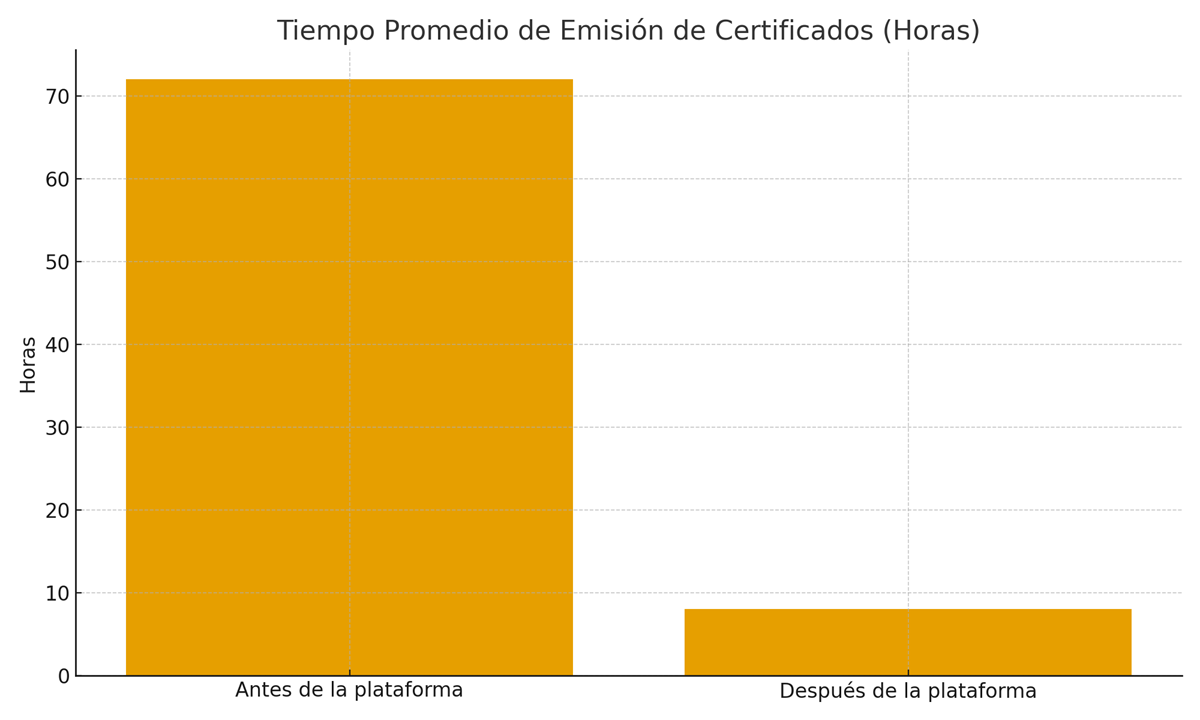
\includegraphics[width=0.48\textwidth]{graphics/emision_certificados.png}
    \caption{Emisión de certificados laborales por mes}
    \label{fig:evolucion_metricas}
\end{figure}

\subsection{Evaluación preliminar}
Con usuarios de prueba, se observó reducción en tiempo de emisión de certificados y consolidación de asistencia, además de menores inconsistencias por duplicidad de archivos \cite{gestion_talento_digital}.